\ifx\wholebook\relax \else

\documentclass[b5paper]{ctexart}
\usepackage[nomarginpar
  %, margin=.5in
]{geometry}

\addtolength{\oddsidemargin}{-0.05in}
\addtolength{\evensidemargin}{-0.05in}
\addtolength{\textwidth}{0.1in}

\usepackage[cn]{../prelude}

\setcounter{page}{1}

\begin{document}

\title{分数}

\author{刘新宇
\thanks{{\bfseries 刘新宇} \newline
  Email: liuxinyu99@hotmail.com \newline}
  }

\maketitle
\fi

\markboth{分数}{数的旅程}

\ifx\wholebook\relax
\chapter{分数}
\fi

\epigraph{此曲只应天上有,人间能得几回闻。}{杜甫《赠花卿》}

2015年9月14日,美国LIGO\footnote{激光干涉引力波}天文台探测到一个神秘信号GW150914。它来自13亿光年之外的一次惊天动地的奇观:一对双黑洞天体彼此靠近、吸引,旋转着合并到一起(如\cref{fig:gravitational-wave})。它们巨大引力激起的“涟漪”穿越13亿年时空\footnote{根据爱因斯坦的广义相对论,引力波以光速传播。}到达了地球。物理学家们花了几个月的事件进行数据分析,排除了可能的干扰因素,最终于2016年2月11日正式宣布:这是人类首次探测到了引力波,证实了爱因斯坦在百年前通过广义相对论做出的预言。LIGO的物理学家们把引力波转换成声音信号,我们得以首次听到来自宇宙深处的“天籁之音”。

\begin{figure}[htbp]
 \centering
 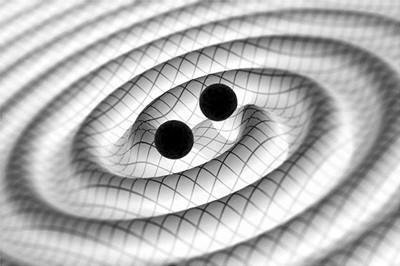
\includegraphics[scale=0.35]{img/gravitational-wave}
 \caption{双黑洞彼此合并过程中产生的引力波示意。}
 \label{fig:gravitational-wave}
\end{figure}

2500年前,正是追寻天籁之音的过程,使得古希腊的先贤毕达哥拉斯发现了音乐背后的数学秘密。相传有一天毕达哥拉斯经过铁匠铺,听到从里面传出了悦耳的声音。这些声音是铁匠们用不同重量的铁锤一起敲打铁砧时产生的。巴洛克时期的音乐家亨德尔有一部作品叫做《快乐的铁匠》(作品编号:HWV430)。毕达哥拉斯注意到有些声音是和谐的,而另一些不和谐。他进一步发现当铁锤的重量比恰好是12、9、8、6时,敲打的声音是和谐的。毕达哥拉斯敏锐地发现了音乐背后的数字规律:

\begin{itemize}
\item 比例$12:6$(即$2:1$)对应纯8度音;
\item 比例$9:6$(即$3:2$)对应纯5度音;
\item 比例$12:9$(即$4:3$)对应纯4度音;
\item 比例$9:8$对应纯2度音。
\end{itemize}

%% \begin{figure}[htbp]
%%  \centering
%%  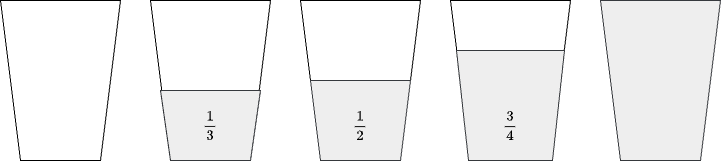
\includegraphics[scale=0.4]{img/cups}
%%  \caption{盛有不同水的杯子}
%%  \label{fig:fraction-cups}
%% \end{figure}

这个故事非常流行,如\ref{fig:pythagoras-music}所示。这幅四联木刻连环画展示了毕达哥拉斯先是聆听到铁匠们挥舞铁锤敲打,然后他开始进行\underdot{定量}研究,包括敲打不同重量的钟,敲打盛有不同水的杯子,弹拨坠有不同重量的琴弦,吹奏不同长度的笛子。但这个故事禁不起推敲,第二幅图和第一幅图是相互矛盾的。我们可以自己动手验证一下。依照第二幅图中的样子,用几个同样的杯子盛上不同的水,然后用不同大小的勺子敲击。我们会发现音调的高低是由杯子而不是勺子决定的。同理,铁匠铺传出的音调高低是由铁砧而不是锤子决定的。但第一幅图中只有一个铁砧。这组连环画还有别的问题。铁锤、钟、杯子、琴弦上的砝码、笛子上的数字4、6、8、9、12、16是印度——阿拉伯数字(见第\ref{sec:hindu-arabic-numerals}节),要到十三、十四世纪才传入欧洲。古希腊的毕达哥拉斯不可能用这样的数字。尽管如此,这组连环画仍然反映了毕达哥拉斯求知好学,善于思考,动手实践进行定量研究的治学传统。

\begin{figure}[htbp]
 \centering
 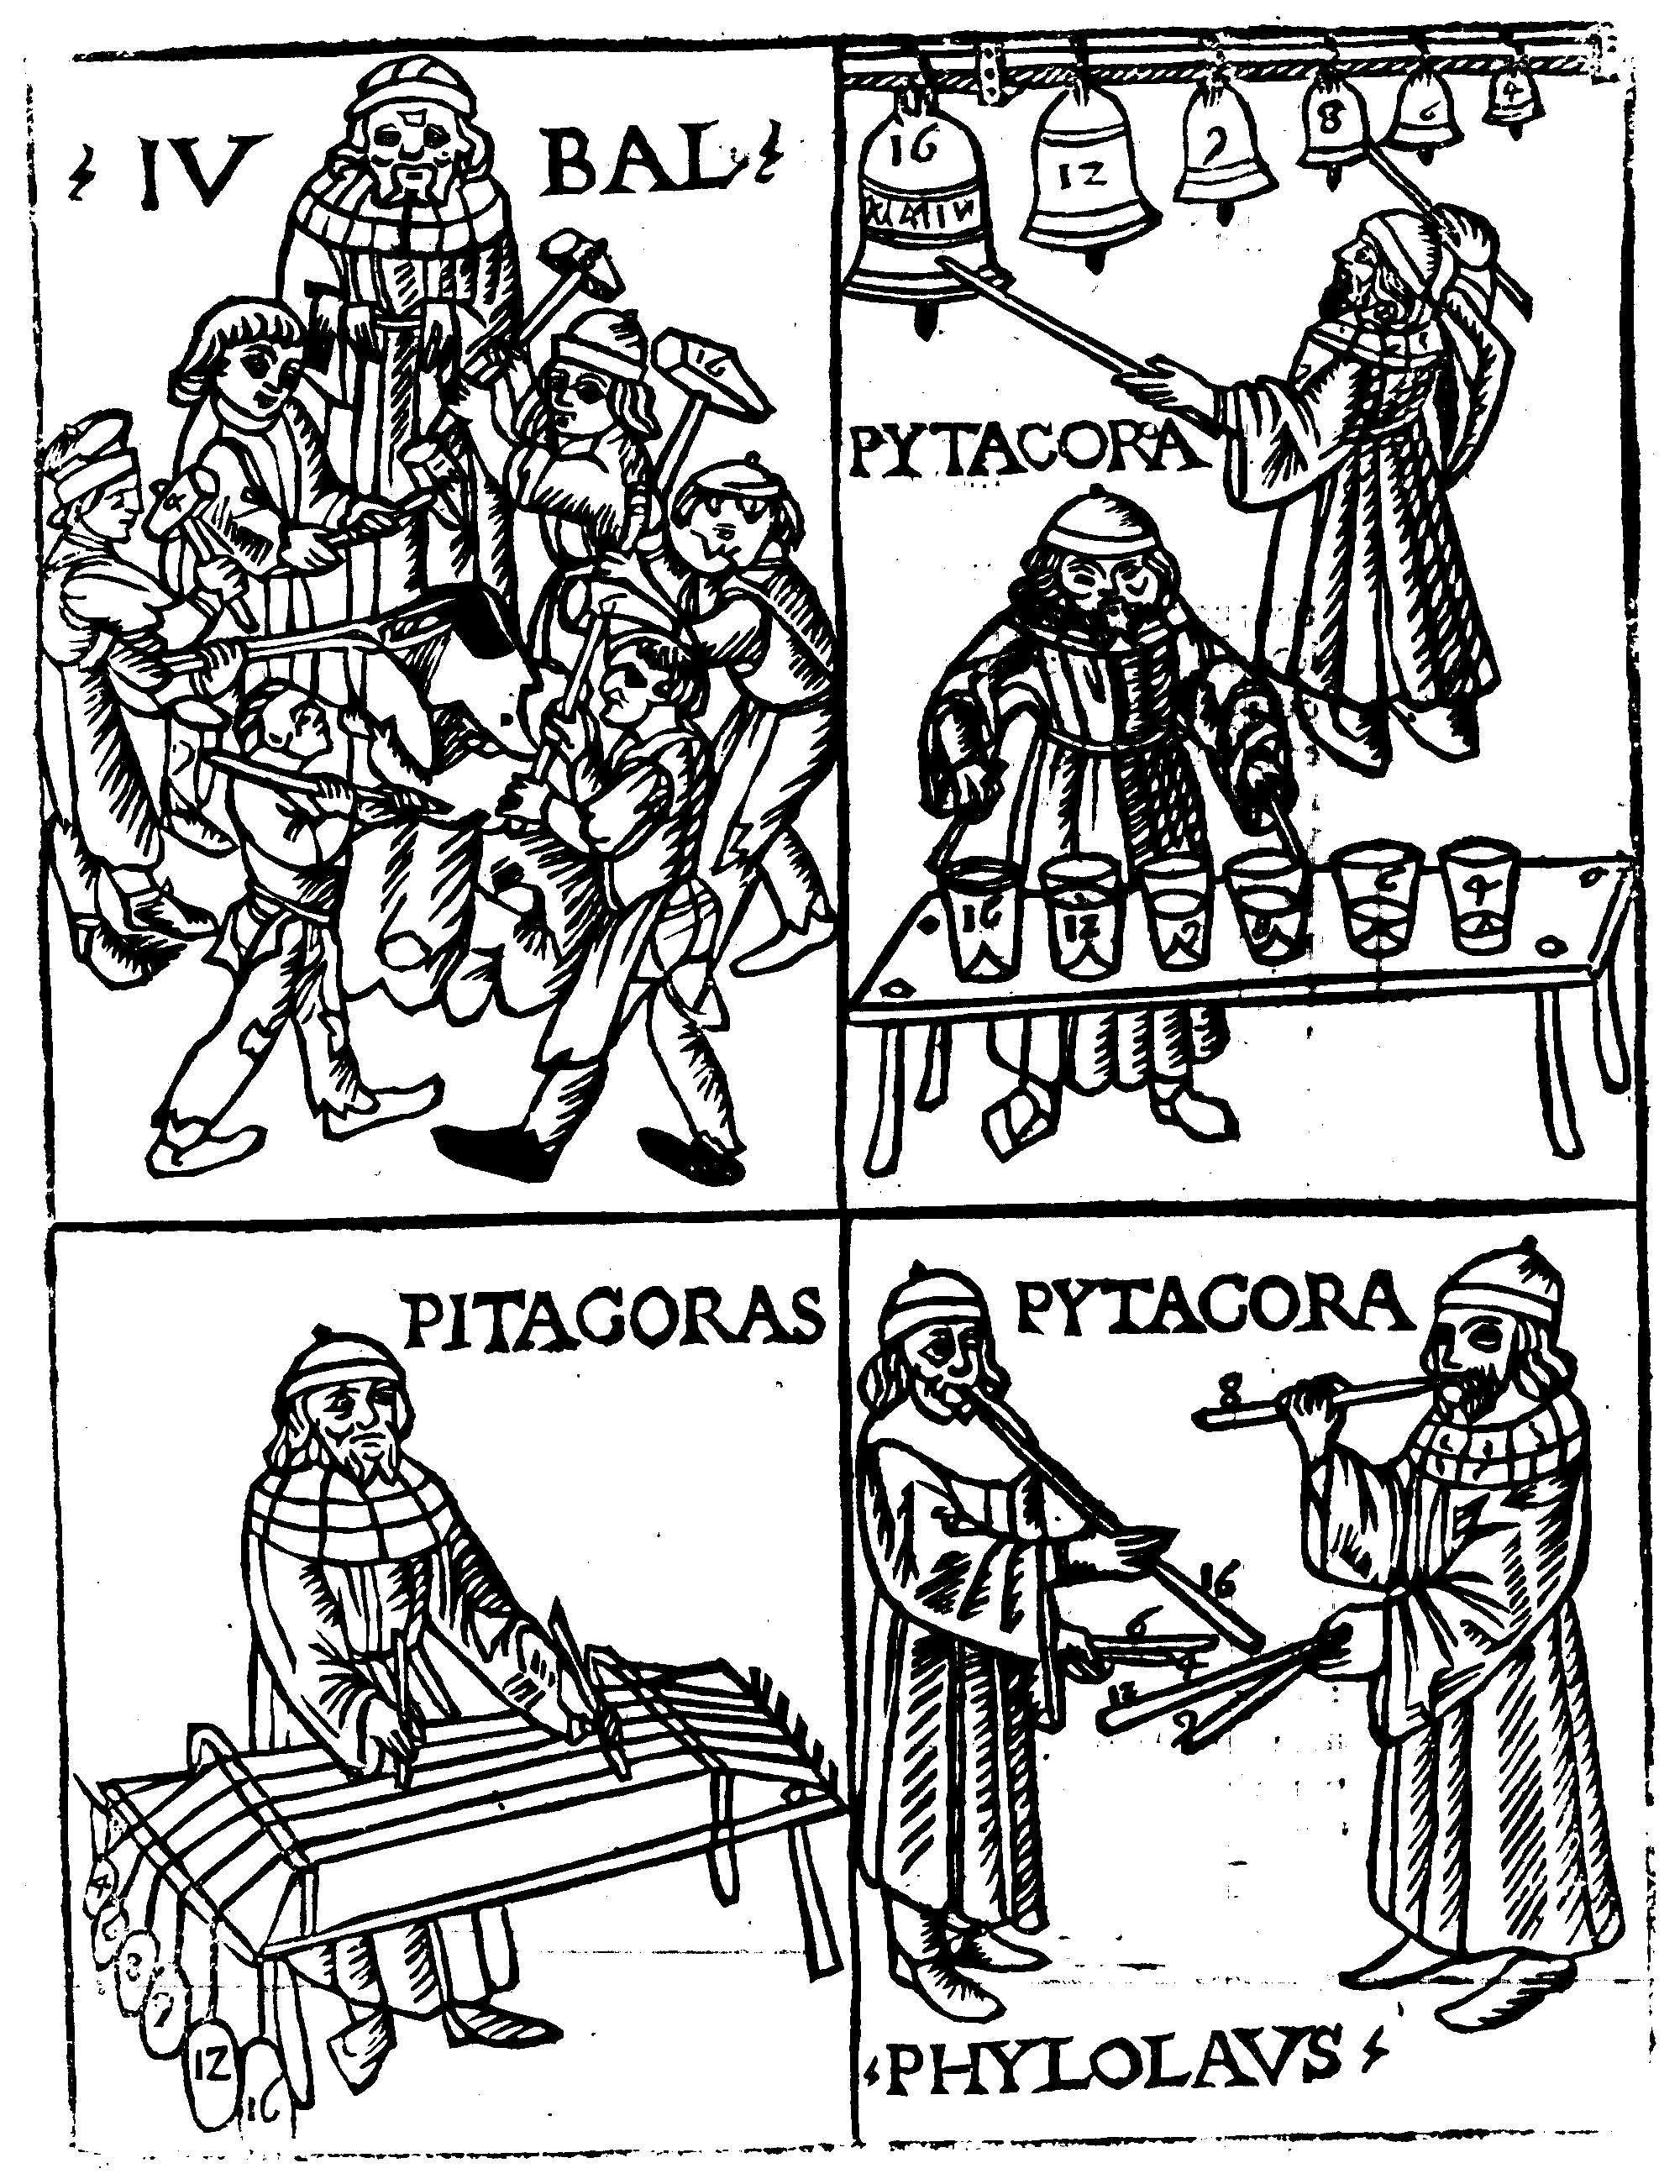
\includegraphics[scale=0.1]{img/pythagoras-music}
 \caption{毕达哥拉斯与音乐,出自1492年(或1480年)弗兰奇诺・加富里奥《乐理》中的木刻插页。}
 %% Woodcut showing Pythagoras with bells, a kind of glass harmonica, a monochord and (organ?) pipes in Pythagorean tuning. From Theorica musicae by Franchino Gaffurio, 1492 (1480?)
 %% https://commons.wikimedia.org/wiki/File:Gaffurio_Pythagoras.png
 \label{fig:pythagoras-music}
\end{figure}

古希腊的乐器叫做里尔琴(Lyre,也译作里拉琴、莱雅琴、诗琴),是一种七弦琴(见\cref{fig:lyre}),在很多场合已经成为代表音乐的符号。我们推测毕达哥拉斯把琴弦的一半,也就是$\frac{1}{2}$张紧弹奏,获得了8度音;把琴弦的$\frac{2}{3}$张紧弹奏,获得了5度音;把琴弦的$\frac{3}{4}$张紧弹奏,获得了4度音;这些音调之间的关系如\cref{fig:octave}所示。

\begin{figure}[htbp]
 \centering
 \subcaptionbox{绘有太阳神阿波罗手持里尔琴的盘子,约公元前480~470年,藏于雅典德尔菲博物馆。\label{fig:lyre}}{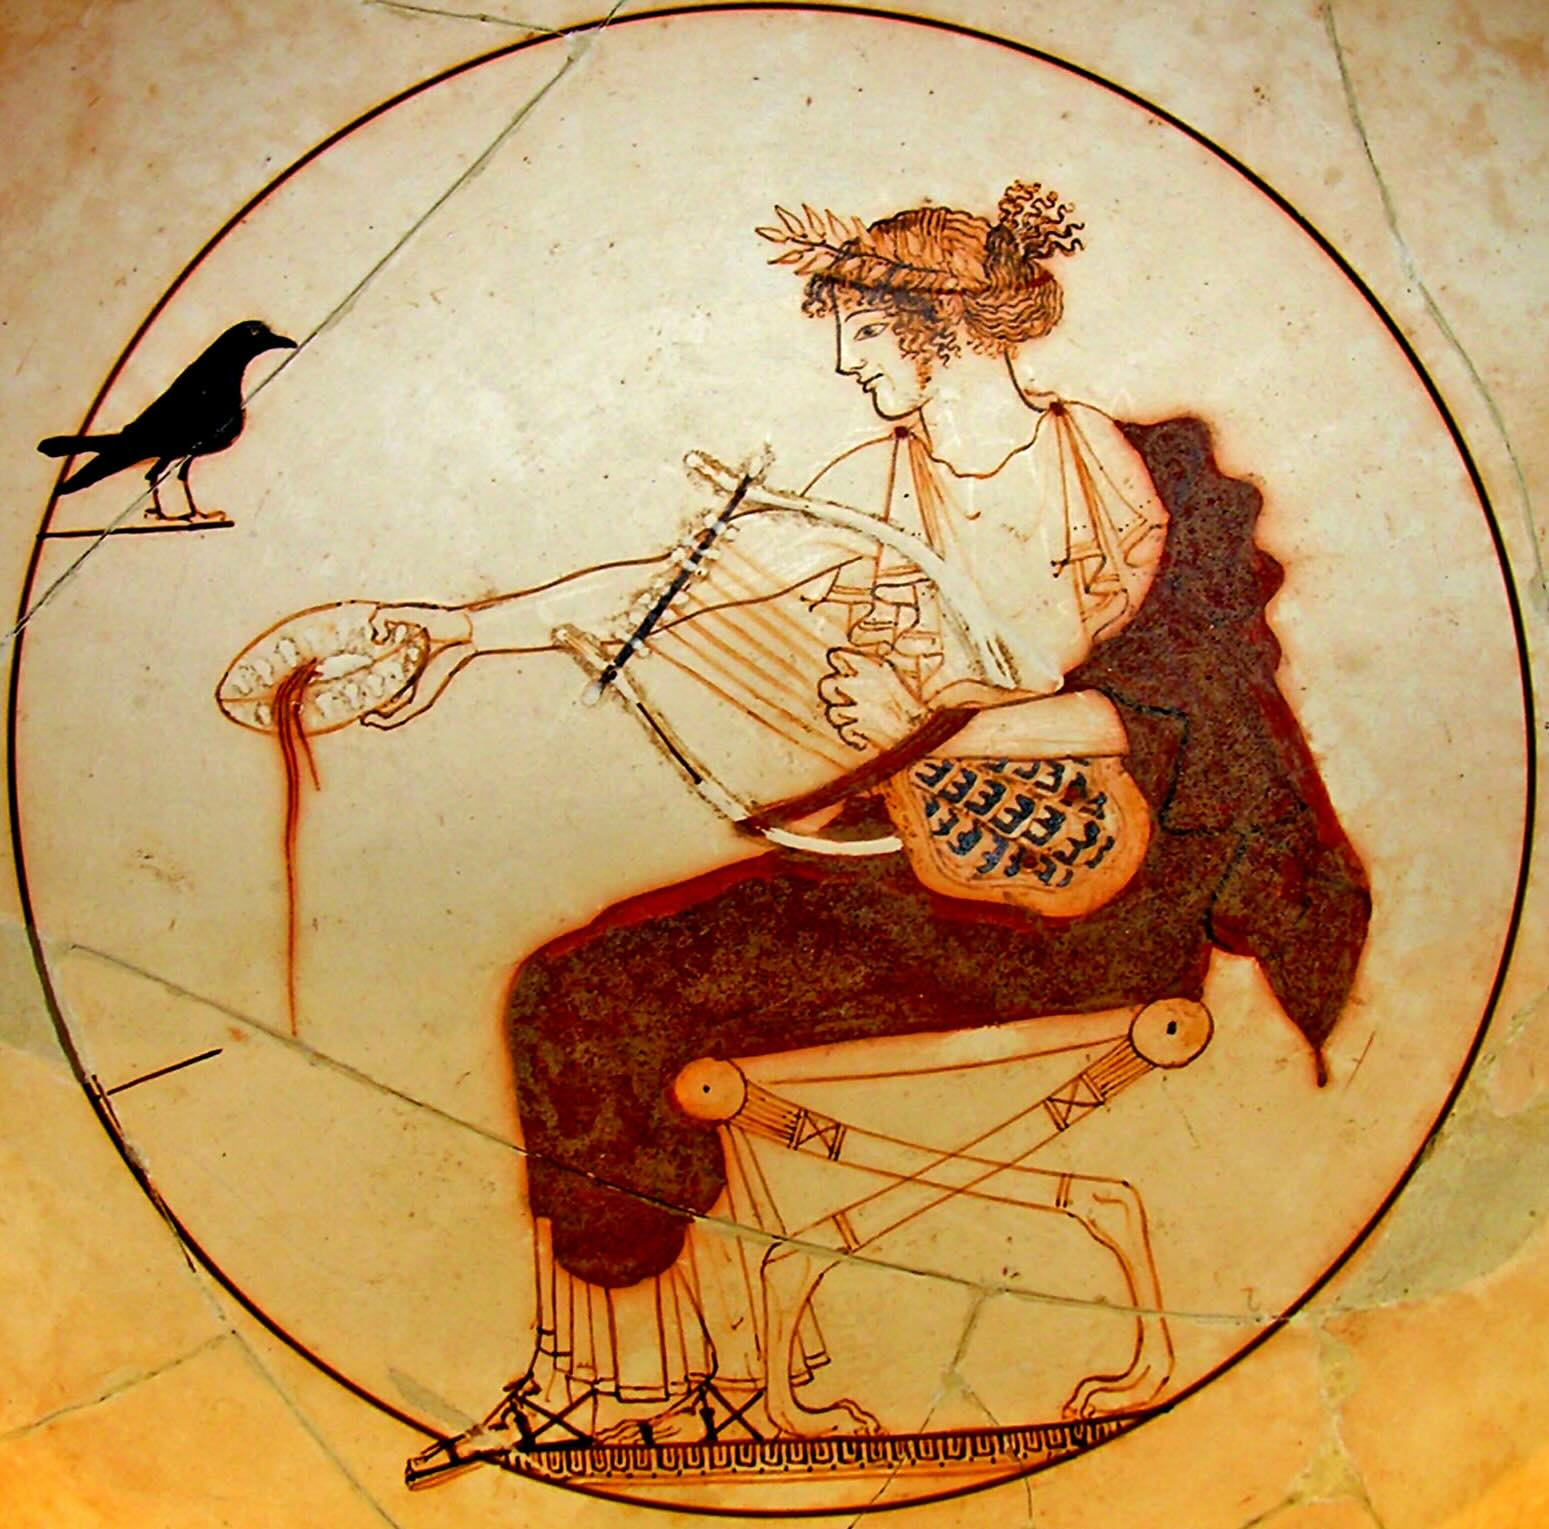
\includegraphics[scale=0.4]{img/apollo-with-lyre}}
 \subcaptionbox{里尔琴符号}{
\includegraphics[scale=0.35]{img/lyre-icon}}
 %% https://www.worldhistory.org/image/986/apollo-with-lyre/
\end{figure}

毕达哥拉斯通过数学,具体说是\underdot{分数与比例}奠定了西方音乐的理论基础。他认为整个宇宙是一把巨大的里尔琴,古希腊人所知道的七个天体(日月和五大行星水星、金星、火星、木星、土星)是琴上的七根弦,在不同的音调上震动。而数与比例代表着宇宙和谐的天籁之音。

\begin{figure}[htbp]
 \centering
 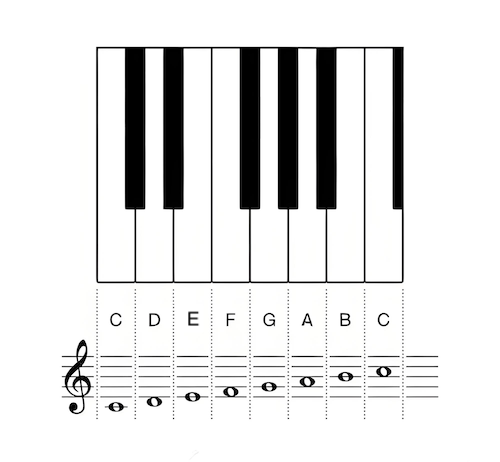
\includegraphics[scale=0.4]{img/octave}
 \caption{两个C间隔8度,琴弦比$2:1$;C与G间隔5度,琴弦比$3:2$;C与F间隔4度,琴弦比$4:3$。}
 \label{fig:octave}
\end{figure}

分数的历史比零和负数还要长。古代中国在春秋时代(公元前770年~前476年)的《左传》中,规定了诸侯的都城大小:最大不可超过周文王国都的三分之一,中等的不可超过五分之一,小的不可超过九分之一。但它们只是表达某种部分的量的词语,而不是真正意义上的分数,因为它们没有直接参与加减乘除运算。古代中国要到汉代才发展出完整的分数计算规则,见\ref{sec:chinese-fractions}节。最早的分数出现在古埃及。

\section{埃及分数}
我们是通过两份重要的古代文件了解到埃及分数的。它们是莱茵德纸草书(见\cref{fig:rhind-papyrus})和莫斯科纸草书(见\cref{fig:moscow-papyrus})。所谓纸草书\footnote{英文Papyrus,是纸的英文paper的字源}是古埃及广泛使用的书写载体。它用当时盛产于尼罗河三角洲的纸莎草的茎制成。经过切片、浸泡、压制、干燥制成。在公元前3000年左右甚至出口到希腊。莎草纸在埃及的干燥气候下可以很好地保存,经历千年而不腐坏。但在潮湿的环境下,很容易霉变损毁。这两份保留了古埃及数学成果的纸草书异常珍贵。它们一份由英国埃及学者莱茵德(Rhind)于1858年购得,现藏于大英博物馆。内容是公元前1650年前后的教科书,作者是书记官阿梅斯\footnote{Ahmes,也译作阿默斯。},包含有85道数学问题。莫斯科纸草书又名戈列尼雪夫纸草书,由俄罗斯贵族戈列尼雪夫于1893年在埃及购得,现藏于莫斯科普希金精细艺术博物馆。作者是约公元前1890年的一位佚名作者,包含有25道数学问题。

\begin{figure}[htbp]
 \centering
 \subcaptionbox{莱茵德纸草书局部\label{fig:rhind-papyrus}}{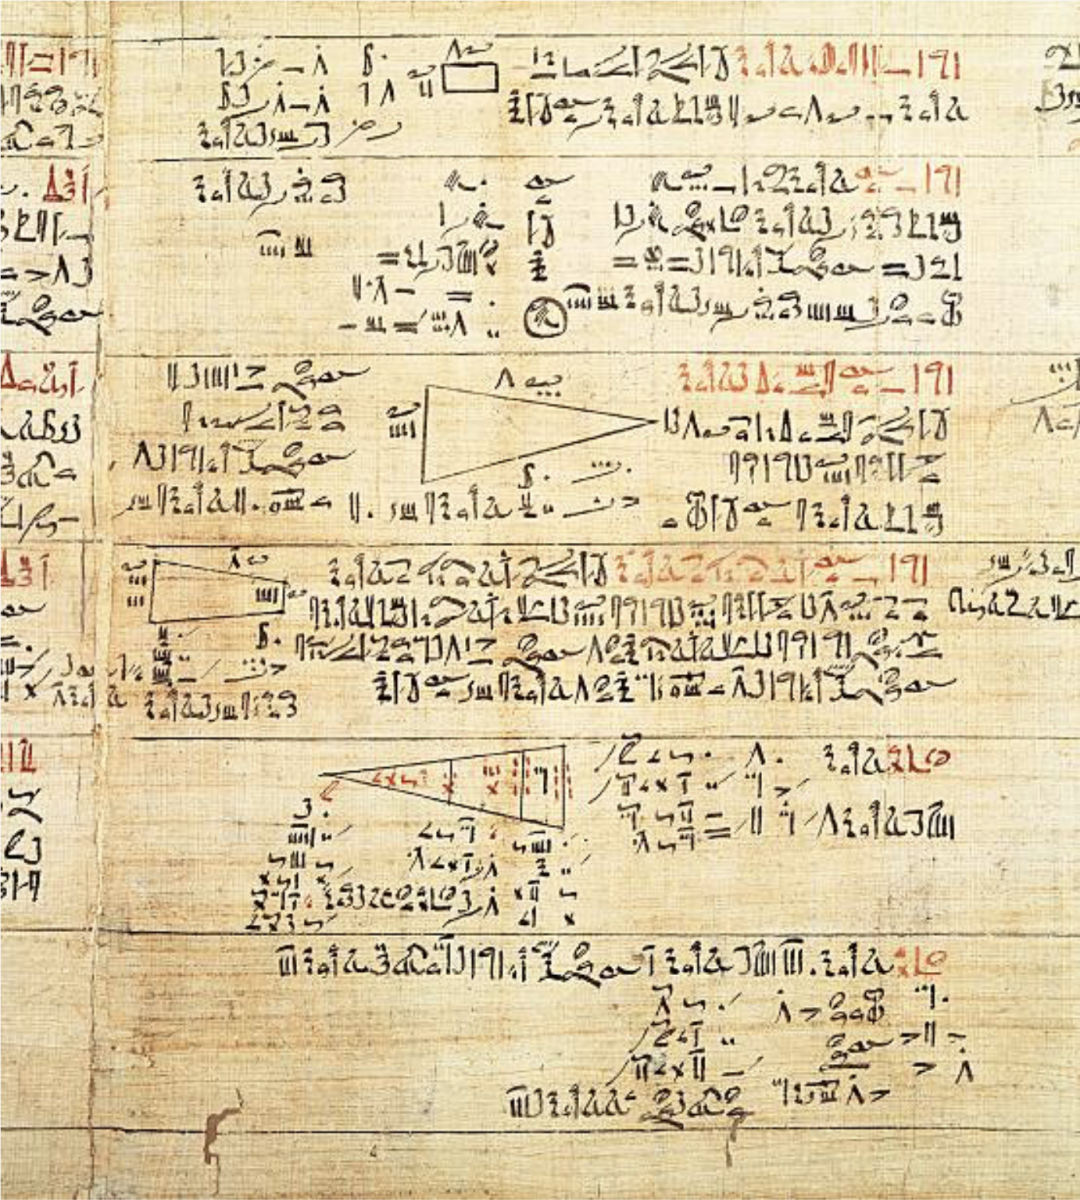
\includegraphics[scale=0.2]{img/rhind-papyrus-part}} \quad
 \subcaptionbox{莫斯科纸草书局部\label{fig:moscow-papyrus}}{ 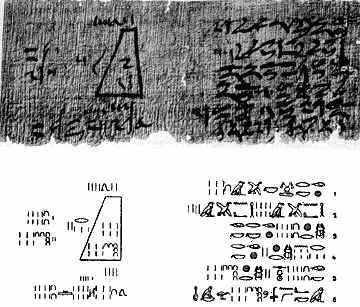
\includegraphics[scale=0.4]{img/moscow-papyrus}}
 %% https://www.britishmuseum.org/collection/image/366139001
 %% https://old.maa.org/press/periodicals/convergence/mathematical-treasure-the-rhind-and-moscow-mathematical-papyri
 %% https://mathshistory.st-andrews.ac.uk/HistTopics/Egyptian_papyri/
\end{figure}

这两份文物反映了古埃及人已使用分数参与运算解决问题。但古埃及的分数有一个既奇怪又合理的特点——所有的分子都是1。因此被称为“单位分数”。在古埃及象形文字(圣书体,见\ref{sec:rosetta-stone}节)中,在数字$a$上方写(画)一个“眼睛”来表示$\frac{1}{a}$,如所\cref{fig:egyptian-fractions}示,表示$\frac{1}{5}$和$\frac{1}{15}$。单位分数的意义是直观易懂的。$\frac{1}{3}$表示把某物均分3份后每份的量,$\frac{1}{5}$是均分5份后每份的量,$\frac{1}{a}$是均分$a$份后每份的量。

\begin{figure}[htbp]
 \centering
 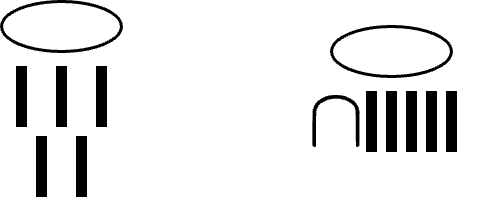
\includegraphics[scale=0.3]{img/egyptian-fractions}
 \caption{埃及分数$\frac{1}{5}$和$\frac{1}{15}$}
 \label{fig:egyptian-fractions}
\end{figure}

但是$\frac{3}{4}$、$\frac{2}{7}$这样的值分子不为1,古埃及人就把它们表示为单位分数之和。例如$\frac{3}{4} = \frac{1}{2} + \frac{1}{4}$,写成象形文字如\cref{fig:sum-egyptian-fractions}左侧所示。中间的符号象征着一个人行走的双腿。如果行走的方向同书写方向一致表示相加,行走的方向同书写的方向相反表示相减。\cref{fig:sum-egyptian-fractions}右侧表示$\frac{2}{5} (= \frac{1}{3} + \frac{1}{15})$。将一个值表示为单位分数的和时,古埃及人要求每个单位分数都不同,不允许重复。因此$\frac{2}{7}$不能写成$\frac{1}{7} + \frac{1}{7}$而要写成$\frac{1}{4} + \frac{1}{28}$。某些情况下,仅仅分解为两个单位分数是不够的。例如莱茵德纸草书上将$\frac{2}{29}$分解为$\frac{2}{29} = \frac{1}{24} + \frac{1}{58} + \frac{1}{174} + \frac{1}{232}$。并且分解方式是不唯一的,例如$\frac{2}{29} = \frac{1}{15} + \frac{1}{435} = \frac{1}{16} + \frac{1}{232} + \frac{1}{464}$。这样的分解没有明显的规律,普通人难以掌握。为此,古埃及人制作了大量的表格以供查找计算。

\begin{figure}[htbp]
 \centering
 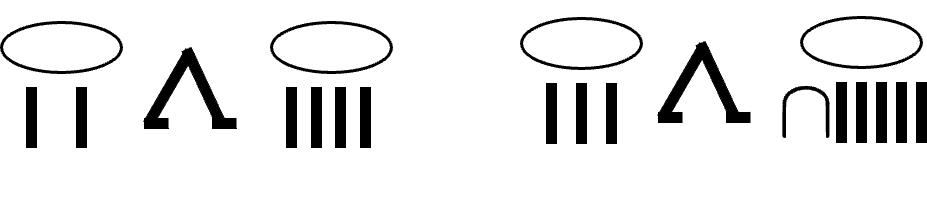
\includegraphics[scale=0.3]{img/sum-egyptian-fractions}
 \caption{左:$\frac{1}{2} + \frac{1}{4}$ \qquad 右:$\frac{1}{3} + \frac{1}{15}$}
 \label{fig:sum-egyptian-fractions}
\end{figure}

迄今为止,没有发现直接的文献,揭示为何古埃及人将分数系统设计为不同的单位分数之和。我们只能加以猜测。有一则传说故事说:老父亲在临终前希望把自己的遗产分给三个儿子。给大儿子$\frac{1}{2}$,二儿子$\frac{1}{3}$,小儿子$\frac{1}{9}$。但全部遗产只是17匹马。三个儿子不知道如何分配,也不愿杀死马进行分割。他们于是去请教村里的长者。老人将自己的一匹马借给了他们。于是大儿子分得$18 \times \frac{1}{2} = 9$匹马,二儿子分得$18 \times \frac{1}{3} = 6$匹马,小儿子分得$18 \times \frac{1}{9} = 2$匹马,剩余$18 - 9 - 6 - 2 = 1$匹马,恰好就是智慧的老人借给他们的那一匹。于是物归原主,老人牵走了他自己的马。这个传说故事用埃及分数解释就是

\[
\frac{17}{18} = \frac{1}{2} + \frac{1}{3} + \frac{1}{9}
\]

尽管脍炙人口,这个传说\underdot{不可能}是古埃及人发展分数系统的初衷。我们在各个民族,包括阿拉伯、印度、犹太、中国的民间故事中都发现了类似的故事。分配的遗产有马、骆驼、大象等动物,数量也有不同。例如三个儿子按照$\frac{1}{2}$、$\frac{1}{4}$、$\frac{1}{6}$分配11个动物,体现为:

\[
\frac{11}{12} = \frac{1}{2} + \frac{1}{4} + \frac{1}{6}
\]

\cref{qn:three-sons}要求给出所有能这样进行分配的数量和比例。我们最早在十八世纪伊朗哲学家纳拉奇(Mulla Muhammad Mahdi Naraqi)的著作中看到此故事的文字记载。其次,尽管在莱茵德纸草书中有关于遗产分配的问题,但主要的分数应用是平均分配。例如第63题\citepage[15]{MKlein-1972}:把700块面包分给四个人,第一人得$\frac{2}{3}$,第二人得$\frac{1}{2}$,第三人得$\frac{1}{3}$,第四人得$\frac{1}{4}$。阿梅斯的解法在我们今天看来相当于解方程\footnote{$\frac{2}{3}$是古埃及极少数特殊的量,不需要写成单位分数之和。}:

\[
\frac{2}{3}x + \frac{1}{2}x + \frac{1}{3}x + \frac{1}{4}x = 700
\]

他把$\frac{2}{3}$、$\frac{1}{2}$ 、$\frac{1}{3}$ 、$\frac{1}{4}$加起来得到$1\frac{3}{4} (= 1 + \frac{1}{2} + \frac{1}{4})$,然后用1除以$1\frac{3}{4}$得$\frac{4}{7} = (\frac{1}{2} + \frac{1}{14})$。最后$700 \times \frac{4}{7} = 400$,从而得到$x = 400$。这相当于我们今天小学高年级的一元一次方程。注意到第一个人和第三个人分得的面包不是整数块。

另一种观点认为,这种分数系统可以用更经济的方式分配物品。考虑将5块面包分给8个人。一种方法是将每个面包平均切分成8份,然后每人拿5块,如\cref{fig:evenly-devide}所示。

\begin{figure}[htbp]
 \centering
 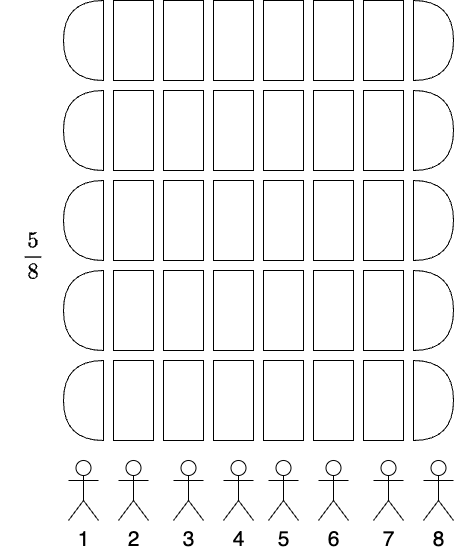
\includegraphics[scale=0.3]{img/evenly-divide}
 \caption{共切成了40小块,每人分得5块。}
 \label{fig:evenly-devide}
\end{figure}

古埃及人可能发现了更好的切割方式,如\cref{fig:egyptian-devide}所示。即每个人拿走一块面包的一半和另一块面包的$\frac{1}{8}$。

\begin{figure}[htbp]
 \centering
 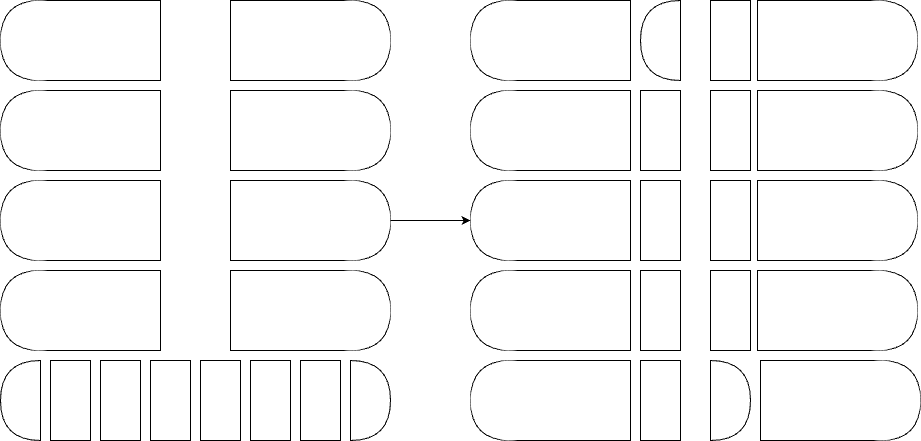
\includegraphics[scale=0.3]{img/egyptian-divide}
 \caption{共切成了16块,每人分得2块(一大$\frac{1}{2}$和一小$\frac{1}{8}$)。}
 \label{fig:egyptian-devide}
\end{figure}

读者朋友们,你觉得古埃及人为何如此设计他们的分数系统呢?以后来的眼光来看埃及分数,一方面它的计算很复杂,逐渐被历史的长河淘汰了,另一方面,数学家思考这样的问题:1)是否每个分数都可以分解成埃及分数?2)如果可以分解,怎样的分解方式最好?其中第一个问题在1202年由斐波那契在《算盘书》中解决了。而第二个问题催生了至今仍未解决的数学猜想。在此之前,我们现看两个相对简单的问题。

\begin{proposition}每个埃及分数都可以分解为两个不同的埃及分数之和,即$\frac{1}{n} = \frac{1}{a} + \frac{1}{b}$。\label{th:egyptian-fraction-split}
\end{proposition}

\begin{proof}
  \begin{align*}
    \frac{1}{n} &= \frac{n+1}{n(n+1)} & \text{上下同}\times (n + 1) & \\
                &= \frac{n}{n(n+1)} + \frac{1}{n(n+1)} && \\
                &= \frac{1}{n+1} + \frac{1}{n(n+1)} && \qedhere
  \end{align*}
\end{proof}

我们可以立即用这个结论推出:

\begin{proposition}
每个$\frac{2}{n}$都能分解为埃及分数。\label{th:decompose-of-2-n}
\end{proposition}

\begin{proof}
  \begin{align*}
    \frac{2}{n} &= \frac{1}{n} + \frac{1}{n} && \\
                &= \frac{1}{n} + \frac{1}{n+1} + \frac{1}{n(n+1)} & \text{上面证明的结论} & \qedhere
  \end{align*}
\end{proof}

当$n$是奇数时,我们能得到更好的结果:$\frac{2}{n}$一定能分解为两个埃及分数:

\begin{proof}
  \begin{align*}
    \frac{1}{n} &= \frac{1}{n+1} + \frac{1}{n(n+1)} & \text{由\cref{th:egyptian-fraction-split}} & \\
    \frac{2}{n} &= \frac{2}{n+1} + \frac{2}{n(n+1)} & \text{左右同} \times 2 & \\
                &= \frac{1}{\frac{1}{2}(n+1)} + \frac{1}{\frac{1}{2}n(n+1)} & n\text{是奇数} &\qedhere
  \end{align*}
\end{proof}

进一步,\cref{qn:unique-decompose-r}要求证明当$n$是奇素数时,这种分解是唯一的。莱茵德纸草书中有一张表记录了从$\frac{2}{5}$到$\frac{2}{101}$的所有分解,印证了这个结论。回到斐波那契证明的定理,考虑任何即约分数\footnote{分子、分母不能进一步约分的分数。}。如果它是假分数,可以先转化成带分数,然后只考虑分解真分数部分。所以只需要证明:

\begin{theorem}[斐波那契]
任何即约真分数$\frac{b}{a}$可分解为埃及分数。
\end{theorem}

\begin{proof}
斐波那契利用带余数的除法:$a = bq + r$,其中$q$是商、$r$是余数,且$0 < r < b$。最接近并小于$\frac{b}{a}$的分数是$\frac{1}{q + 1}$。斐波那契考虑
\[
  \frac{b}{a} = \frac{1}{q + 1} + x
\]
然后再把$x$分解为埃及分数。通过这一分而治之的思想,原来的问题就转化为分解$x$的问题。
\begin{align*}
  x & = \frac{b}{a} - \frac{1}{q + 1} = \frac{bq + b - a}{a(q + 1)} & \text{通分} \\
    & = \frac{b - (a - bq)}{a(q+1)} = \frac{b - r}{a(q+1)} & \text{余数}r = a - bq
\end{align*}
注意到$x$的分子$b' = b - r$。由于余数$0 < r < b$,所以$b' < b$,它比原分数$\frac{b}{a}$的分子$b$至少减小了1。如果$b' = 1$,则分解完成,否则我们继续分解$x$。这样就可以得到一系列不断缩小的分子序列$b > b' > b'' > \cdots$因为$b$是一个确定的正整数,它不会无限减小,所以必定在某次达到1从而结束分解。因此每个即约真分数都可以分解为埃及分数。
\end{proof}

我们用一个例子$\frac{5}{11}$来理解斐波那契的证明。$11 = 2 \times 5 + 1$,商$q = 2$、余数$r = 1$。第一步分解:

\begin{align*}
\frac{5}{11} & = \frac{1}{q + 1} + x = \frac{1}{3} + x  \\
 x &= \frac{5}{11} - \frac{1}{3} = \frac{4}{33} \\
\frac{5}{11} &= \frac{1}{3} + \frac{4}{33}
\end{align*}

接下来分解$\frac{4}{33}$。再次用带余数除法$33 = 4 \times 8 + 1$,商$q = 8$、余数$r = 1$。

\begin{align*}
\frac{4}{33} & = \frac{1}{q + 1} + x = \frac{1}{9} + x  \\
 x &= \frac{4}{33} - \frac{1}{9} = \frac{12 - 11}{99} = \frac{1}{9}
\end{align*}

分解结束,得到:
\[
\frac{5}{11} = \frac{1}{3} + \frac{1}{9} + \frac{1}{99}
\]

斐波那契使用的策略是每次用\underdot{最接近}原分数$\frac{b}{a}$的埃及分数进行分解。这种策略叫做\underdot{贪心策略}。但是贪心策略并不一定给出最优分解。例如

\[
\frac{5}{121} = \frac{1}{25} + \frac{1}{757} + \frac{1}{763309} + \frac{1}{873960180913} + \frac{1}{1527612795642093418846225}
\]

但还有另一个分解:
\[
\frac{5}{121} = \frac{1}{33} + \frac{1}{121} + \frac{1}{363}
\]

所谓最优的含义是:用\underdot{最少}的埃及分数分解,如果两个分解的埃及分数个数相同,则分母越小越好。练习X提供了用贪心策略分解埃及分数的计算机程序。斐波那契的方法每次至少将分子减1,所以$\frac{b}{a}$最多一定被分解为$b$个埃及分数,但$\frac{5}{11}$的例子说明可能存在着更好的分解方法。匈牙利数学家保罗·埃尔德什和德国数学家斯特劳斯在1950年猜想对于大于1的自然数$n$,

\[
\frac{4}{n} = \frac{1}{a} + \frac{1}{b} + \frac{1}{c}
\]
总成立,其中$a > b > c$。也就是说$\frac{4}{n}$总能分解为3个两两不同的埃及分数。这个著名的数论问题称为埃尔德什——斯特劳斯猜想\footnote{Erdős - Straus},迄今(2015)仍未解决。
% https://mathworld.wolfram.com/Erdos-StrausConjecture.html

\section{古巴比伦的分数}
以今天的眼光来看,埃及分数不便于计算,像是在数学上走了一段弯路。它的形式意义大于它的实用意义。此后的古希腊、古罗马并未发展出独立的分数系统,而是用一些特定的词汇表示部分的量。古罗马表示部分的词汇来源于其重量单位系统。单位重量叫做as,它的$\frac{1}{12}$叫做uncia,是英制重量盎司ounce的词源。\cref{tab:roman-fractions}列出了常用的罗马分数名词:

% https://mathshistory.st-andrews.ac.uk/Miller/mathsym/fractions/
\begin{table}
  \centering
  \begin{tabular}{|c|l|l||c|l|l|}
  \hline
  值 & 词汇 & 意义 & 值 & 词汇 & 意义 \\
  \hline
  $\frac{1}{12}$ & uncia    & 十二分之一 & $\frac{9}{12}$ & dodrans    & 去掉四分之一 \\
  \hline
  $\frac{2}{12}$ & sextans  & 六分之一 & $\frac{10}{12}$ & dextans   & 去掉六分之一 \\
  \hline
  $\frac{3}{12}$ & quadrans & 四分之一 & $\frac{11}{12}$ & deunx    & 去掉一个uncia \\
  \hline
  $\frac{4}{12}$ & triens   & 三分之一 & $\frac{1}{24}$ & semuncia   & uncia的一半  \\
  \hline
  $\frac{5}{12}$ & quincunx & 五个uncia & $\frac{1}{48}$ & sicilicus &  \\
  \hline
  $\frac{6}{12}$ & semis    & 一半    & $\frac{1}{72}$ & scriptulum    &  \\
  \hline
  $\frac{7}{12}$ & septunx  & 七个uncia & $\frac{1}{144}$ & scripulum  &  $\frac{1}{12} \times \frac{1}{12}$ \\
  \hline
  $\frac{8}{12}$ & bes      & 三分之二 & $\frac{1}{288}$ & scrupulum    &  $\frac{1}{24} \times \frac{1}{12}$\\
  \hline
  \end{tabular}
  \caption{罗马分数名称}
  \label{tab:roman-fractions}
\end{table}

有许多词至今仍影响着我们的语言,如表示$\frac{1}{2}$的semi,常用作“半”的词根。例如半圆semicircle、分号semicolon、半导体semiconductor等。表示$\frac{1}{4} = \frac{3}{12}$的quadrans在英语中是quarter,仍表示一刻钟、一季度。

古巴比伦发展出了分数系统。我们从耶鲁大学收藏的一块泥板中找到了“物证”,如\cref{fig:babylonian-yale}所示。此图描绘了一个正方形和对角线。正方形的一边刻有楔形文字30(右上角的3个楔形),在对角线下刻有文字42, 25, 35,贯穿着这同一对角线还刻有文字1, 24, 51, 10。我们在初中数学课上学到过正方形的对角线长度是边长的$\sqrt{2}$倍。简单计算$30 \times \sqrt{2} \approx 30 \times 1.4142 = 42.426$,其中42恰好是对角线下刻的文字的第一个。古巴比伦人使用60进制,我们怀疑接下来的25, 35是小数部分。这很容易验证:

\begin{figure}[htbp]
 \centering
 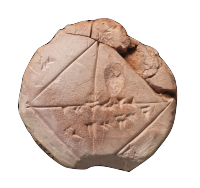
\includegraphics[scale=0.8]{img/babylonian-yale}
 \caption{耶鲁大学古巴比伦泥板,编号Y7289}
 \label{fig:babylonian-yale}
\end{figure}

\[
\frac{25}{60} + \frac{35}{60^2} \approx 0.4264
\]

这说明古巴比伦人正确地计算出了对角线长度。42, 25, 35代表$42.426 \approx 30 \times \sqrt{2}$。那么1, 24, 51, 10会不会也是个小数呢?我们试一试:

\[
1 + \frac{24}{60} + \frac{51}{60^2} + \frac{10}{60^3} \approx 1.414213
\]

竟然是$\sqrt{2}$的小数表示,并且精度达到了百万分位(小数点后6位)!我们由此确知古巴比伦人发展出了60进制小数系统。但由于没有小数点,他们的数字是有歧义的。例如12, 15既可能是$12 \times 60 + 15 = 720$也可能是$12 + \frac{15}{60} = 12.25$。再加上0没有被统一使用,我们只能通过上下文加以猜测一个数的真正含义。

由于使用60进制,古巴比伦人可以比较精细、准确地表示$\frac{1}{60}$~$\frac{59}{60}$之间的部分量。当使用2到3位60进制小数时,已足够生产、生活、乃至天文观测所需的精度。此外,60的真因数\footnote{除1和$n$以外的因数称$n$的真因数。}足够丰富(包括2, 3, 4, 5, 6, 10, 12, 15, 20, 30),除不尽产生循环小数的机会较少(10进制只有2和5两个真因数,只有少数情况能除尽而不循环,参见第X.X节)。可能由于这些因素,古巴比伦人只使用60进制小数而没有发展出一般的分数系统。

\section{古代中国的分数}
\label{sec:chinese-fractions}

在汉代的《九章算术》中,已经包含了分数四则运算规则和各种应用题。这些内容集中出现在第一卷“方田”中(见\cref{fig:jiuzhang})。由于篇幅不大,我们不妨一起赏析一下中国古人的智慧。首先是分数的记法。《九章算术》中已经使用了“a分之b”这样的描述,和现代汉语完全一致,如:“十五分之一”。古人用步数表示长度,例如一块田长九步、宽五步。当用分数表示长度时,说“a分步之b”,如:“七分步之四”、“五分步之三”。而在现代汉语中,我们说七分之四步、五分之三步。又如表示金额:“八钱三分钱之一”,可见已经有了带分数的概念。对应现代汉语中的八又三分之一钱。《九章算术》中的分数直接来源于除法,如:“七人卖四马,一人卖七分马之四。”这就是$\frac{4}{7}$的意义。

\begin{figure}[htbp]
 \centering
 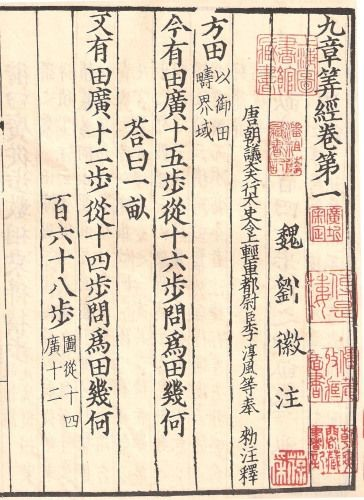
\includegraphics[scale=0.4]{img/jiuzhang}
 \caption{《九章算术》书影}
 \label{fig:jiuzhang} % The Nine Chapters on the Mathematical Art
\end{figure}


有了分数记法,接下来《九章算术》要处理一个分数的值是否“唯一”的问题。这就引出了“约分”的概念。作者用两道例题说明:
\begin{enumerate}[1)]
\item 今有十八分之十二,问约之得几何?答曰:三分之二。(即:$\frac{12}{18} = \frac{2}{3}$)
\item 又有九十一分之四十九,问约之得几何?答曰:十三分之七。(即:$\frac{49}{91} = \frac{7}{13}$)
\end{enumerate}

具体怎样约分呢?《九章算术》给出了“辗转相除”法,即著名的欧几里得算法求最大公约数(也叫做最大公因数):“可半者半之;不可半者,副置分母、子之数,以少减多,\underdot{更相减损},求其等也。以等数约之。”解释成现代汉语:首先是特殊情况。若分子分母都是偶数,先不断$\div 2$,化为奇数。然后是一般情况。记分数为$\frac{b}{a}$,记$a$与$b$的最大公约数为$(a, b)$,则:

\be
\label{eq:gcd-minus}
(a, b) = \begin{cases}
  a > b :& (a - b, b) \\
  a = b :& a \\
  a < b :& (a, b - a)
  \end{cases}
\ee

就是“以少减多,更相减损、求其等也”的意思。这种方法在欧几里得的《几何原本》中有系统的描述和正确性证明,今天被称做“欧几里得算法”,在中国常被称做辗转相除法。对比一般的方法:把$a$、$b$分解为因子的积,然后找出最多的公因子相乘,欧几里得算法的效率极高\footnote{利用除法代替\cref{eq:gcd-minus}中的减法可以达到“对数复杂度”。100位的整数,大约递归8次左右即可算出。},便于机械化计算,是当今数论和密码学的基础算法\footnote{在抽象代数,如环论、域论中也有重要应用}。我们将在下一章中详细介绍它的原理。这里举一个例子:求18和12的最大公约数。

\[
(18, 12) = (18 - 12, 12) = (6, 12) = (6, 12 - 6) = (6, 6) = 6
\]

只用了3步就求出了结果。最后分子分母同除以最大公约数得:$\frac{12}{18} = \frac{12/6}{18/6} = \frac{2}{3}$。

《九章算术》接下来通过例题引入分数加法:

\begin{enumerate}[1)]
\item 今有三分之一,五分之二,问合之得几何?答曰:十五分之十一。(即:$\frac{1}{3} + \frac{2}{5} = \frac{11}{15}$)
\item 又有三分之二,七分之四,九分之五,问合之得几何?答曰:得一、六十三分之五十。(即:$\frac{2}{3} + \frac{4}{7} + \frac{5}{9} = 1\frac{50}{63}$)
%% \item 又有二分之一,三分之二,四分之三,五分之四,问合之得几何?答曰:得二、六十分之四十三。(即:$\frac{1}{2} + \frac{2}{3} + \frac{3}{4} + \frac{4}{5} = 2\frac{43}{60}$)
\end{enumerate}

作者解释分数加法原理:“母互乘子,并以为实。母相乘为法。”即:

\be
\frac{b}{a} + \frac{d}{c} = \frac{bc + ad}{ac}
\ee

新的分子叫“实”,分母叫“法”。接下来:“实如法而一。不满法者,以法命之。”即$\frac{n}{n} = 1$,抽取整数部分化为带分数。最后说:“其母同者,直相从之。”即:

\be
\frac{b}{a} + \frac{c}{a} = \frac{b + c}{a}
\ee

分母相同时,直接将分子相加。可见《九章算术》的通分并未使用最小公倍数,而是直接将分母相乘。

《九章算术》接下来介绍分数减法,基本上类似于加法,我们省略跳过。之后介绍分数大小的比较。《九章算术》的作者采用和减法一样的处理,通过母子互乘比大小。即将$\frac{b}{a}$与$\frac{d}{c}$的大小比较转化为$bc$与$ad$的大小比较。接下来在介绍多个分数的平均数之后讲解分数除以整数,例如:“今有七人,分八钱三分钱之一。问人得几何?答曰:人得一钱二十一分钱之四。”即$8\frac{1}{3} \div 7 = 1\frac{4}{21}$。作者解释说:“以人数为法,钱数为实,实如法而一。有分者通之。”即用金额作分子,人数作分母。这里并没有考虑除数是分数的情况。最后是分数乘法:

\begin{enumerate}[1)]
\item 今有田广七分步之四,从五分步之三,问为田几何?答曰:三十五分步之十二。(即:$\frac{4}{7} \times \frac{3}{5} = \frac{12}{35}$)
\item 又有田广九分步之七,从十一分步之九,问为田几何?答曰:十一分步之七。(即:$\frac{7}{9} \times \frac{9}{11} = \frac{7}{11}$)
%% \item 又有田广五分步之四,从九分步之五,问为田几何?答曰:九分步之四。(即:$\frac{4}{5} \times \frac{5}{9} = \frac{4}{9}$)
\end{enumerate}

作者给出的计算规则是:“母相乘为法,子相乘为实,实如法而一。”即分子分母相乘再化带分数。有趣的是《九章算术》对带分数乘法进行了单独处理:

\begin{enumerate}[1)]
\item 今有田广三步三分步之一,从五步五分步之二,问为田几何?答曰:十八步。(即:$3\frac{1}{3} \times 5\frac{2}{5} = 18$)
\item 又有田广七步四分步之三,从十五步九分步之五,问为田几何?答曰:一百二十步九分步之五。(即:$7\frac{3}{4} \times 15\frac{5}{9} = 120\frac{5}{9}$)
%% 又有田广十八步七分步之五,从二十三步十一分步之六,问为田几何?答曰:一亩二百步十一分步之七。
\end{enumerate}

作者解释说:“分母各乘其全,分子从之,相乘为实。分母相乘为法。实如法而一。”即化成假分数,相乘再化带分数。例如:

\[
3\frac{1}{3} \times 5\frac{2}{5} = \frac{10}{3} \times \frac{27}{5} = \frac{10 \times 27}{3 \times 5} = 18
\]

《九章算术》一开篇就系统地引入了分数及其四则运算。可见中国古人对分数的重视。后继的各种图形面积、方程计算都建立在这个基础上。

\section{印度分数和小数}

我们今天使用的分数记法源自古印度。印度人将表示分子的数写在上方,将表示分母的数写在下方,但并未使用分数线,如:

\begin{align*}
  3 \\
  4
\end{align*}

表示四分之三。后来阿拉伯人在约公元1200年引入了分数线来分开分子与分母\cite{Pumfrey-2011},如:

\[
\dfrac{3}{4}
\]

斐波那契最早将现代分数记法介绍到欧洲,但在写带分数时,他照搬了阿拉伯人从右向左的书写习惯,将分数写在整数的左边\cite{Miller-2025}。分数线带来了不小的印刷困难。在1718年,英国著名的川宁茶叶公司创世人托马斯·川宁\footnote{Thomas Twining}在记账时用斜线代替水平分数线,如:1/4磅茶叶。这样就便于印刷和用打字机书写分数。今天很多字处理和编辑软件可以方便输入分数。不少网页支持了 \LaTeX 排版,可以用\lstinline|\frac{b}{a}|来输入$\frac{b}{a}$。

随着印度——阿拉伯计数系统的确立,阿拉伯学者开始引入了十进制小数。数学家阿尔·卡西(Al-Kashi,公元920年~980年)在他的著作《圆周的研究》\footnote{{\em al-Risali al-mohitije}译作英文{\em Treatise on the circumference}}中将圆周率$\pi$的值写为:“sah-hah 3 14159”,其中sah-hah的意思是整数部分(今天土耳其语中的sahih),修饰了3,接下来是小数部分。可见此时尚未引入小数点。中国魏晋时的数学家刘徽(见\cref{fig:liuhui})在注解《九章算术》时,不满于古代用3作为圆周率,于是:“微数无名知以为分子,以十为分母”,决定采用十进分数来求得更精确的值。当他用正96边形逼近圆时求得:“三百一十四寸六百二十五分寸之一百六十九”,这个值的表示已经非常接近小数的形式了\footnote{关于这个值,刘徽接着写道:“则出圆之表矣。故还就一百九十二觚之全幂三百一十四寸以为圆幂之定率而弃其余分。”他觉得大了,故得到此时的圆周率3.14。但他不甘心,又继续用192边形计算到“三百一十四寸二十五分寸之四”。这个带分数是$314\frac{4}{25} = 314.16$寸。可见刘徽是混合使用小数和分数的。}。

\begin{figure}[htbp]
 \centering
 \subcaptionbox{纳皮尔肖像,1616年油画,爱丁堡大学收藏\label{fig:napier}}{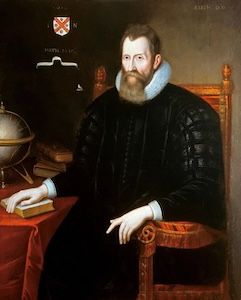
\includegraphics[scale=0.5]{img/napier}} \quad
 % https://www.britannica.com/biography/John-Napier
 \subcaptionbox{蒋兆和创作的刘徽像,部编数学课本\label{fig:liuhui}}{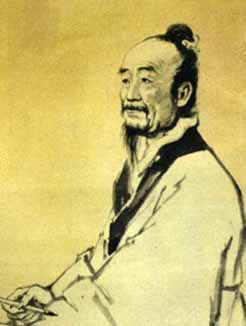
\includegraphics[scale=0.46]{img/liuhui}}
 % https://wapbaike.baidu.com/tashuo/browse/content?id=b1fc49ab180770763a28420d
\end{figure}

1530年,鲁道夫(Christoff Rudolff,1499?~1545?年 )使用一条数线分隔整数和小数部分。后来马吉尼(Magini,1555年~1617年)将竖线改进成了小数点,但并未得到广泛使用。直到20年后英国学者约翰·纳皮尔(John Napier,1550年~1617年,见\cref{fig:napier})发明对数时使用了小数点,现代小数形式才被广泛接受。我们常用的百分数符号\%是佚名的某位意大利人在1425年引入的。

从另一角度看,小数是分母为10、100、1000……的分数的和。百分数看似是分母为100的分数,实则只是小数乘以100的结果。这是因为百分数的分子不一定是整数。例如某网站说它的可靠性非常高,达99.999\%(俗称5个9),这相当于小数0.99999。在日常生活中,人们还会用千分数,写作999.99\textperthousand。在金融领域还会用基点(BPS:base points的缩写)这个量。1bps = 0.01\% = 0.0001。比如我们看见新闻说美联储(美国联邦储备委员会,是美国的中央银行的核心管理机构)宣布降息25个基点。实际上就是降低利息0.25\% = 0.0025。例如利率从2.5\%降低25个基点就变成2.5\% - 0.25\% = 2.25\%。

现在我们回过头来说为何小数是分母为10、100、1000……的分数和?并提出一个问题:是否每个分数都可以\underdot{唯一}地表示成小数?举例来说0.125 = $\frac{1}{10} + \frac{2}{100} + \frac{5}{1000}$,恰好是分母为10的$\frac{1}{10}$,分母为100的$\frac{2}{100}$,分母为1000的$\frac{5}{1000}$的和。一般来说,小数$0.a_1 a_2 \dots a_n$可表示为:

\be
a_1 \frac{1}{10} + a_2 \frac{1}{100} + \cdots + a_n \frac{1}{10^n}
\label{eq:decimal-as-sum}
\ee

我们在数学课上知道,小数分为有限小数(如0.125)和无限小数(如$0.\dot{3} = 0.333\cdots, 0.\dot{1}\dot{5} = 0.1515\cdots, \pi = 3.14159\cdots$)。根据\cref{eq:decimal-as-sum},无限小数可写成无限个分数的和。那么这无限个正数的和是个有限值还是无限大?为了解答这个问题,我们线引入一个看似反直觉的命题:

\begin{lemma}
  无限循环小数$0.999\cdots$的值是1。
\end{lemma}

乍看上去左边的$0.999\cdots$和右边的1明显是两个不同的数,它们怎么会相等呢?

\begin{proof}
  令$x = 0.999\cdots$,扩大10倍:$10x = 9.999\cdots$,相减:
  \begin{align*}
    10x - x &= 9.999\cdots - 0.999\cdots && \\
         9x &= 9 & \text{右侧的小数部分减光了} & \\
          x &= 1  && \qedhere
  \end{align*}
\end{proof}

注意,小数部分只有有限个9时等号不成立,哪怕有$n = 10000$个9。因为$9.99\cdots9$(个位的9和小数部分的9999个9)减$0.99\cdots9$(小数部分的1万个9)等于$8.99\cdots91$。因此$x = \frac{8.99\cdots91}{9} \ne 1$。即1万位有限小数$0.99\cdots9 \ne 1$。这样无限个正数的和$\frac{9}{10} + \frac{9}{100} + \cdots = 1$,是个确定的有限值\footnote{我们也可以用高中数学的极限概念进行证明。注意到$n$位有限小数:$0.99\cdots9 = 1 - 0.00\cdots01 = 1 - \frac{1}{10^{n+1}}$,所以$0.999\cdots = \lim\limits_{n\to\infty} (1 - \frac{1}{10^{n+1}}) = 1 - \lim\limits_{n\to\infty} \frac{1}{10^{n+1}} = 1 - 0 = 1$。}。

\begin{corollary}
  把任何无限小数$0.a_1a_2\cdots$写成无穷多个分数的和:$a_1 \dfrac{1}{10} + a_2 \dfrac{1}{100} + \cdots$这个和是有限的。
\end{corollary}

\begin{proof}
  由于每个小数位$0 \leq a_i \leq 9$,所以
  \begin{align*}
0 \leq 0.a_1 a_2 \cdots = a_1\frac{1}{10} + a_2\frac{1}{10^2} + \cdots \leq \frac{9}{10} + \frac{9}{10^2} + \cdots = 0.999\cdots = 1 & \qedhere
  \end{align*}
\end{proof}

\section{数系的扩展}

数学家小传:埃尔德什。

\begin{Exercise}[label={ex:fractions}]
\Question{找出三个儿子按照$\frac{1}{a}$、$\frac{1}{b}$、$\frac{1}{c}$分配$n$个动物的所有可能数值和比例。要求大儿子分得的财产多于二儿子,二儿子分得的财产多于小儿子。恰好借来一只动物后可以分好并余下一只动物。\label{qn:three-sons}}
\Question{如果你会编程,请用计算机枚举上面的所有解。}
\Question{$\bigstar$若$p$为大于2的素数,证明$\frac{2}{p}$可\underdot{唯一}分解为两个埃及分数$\frac{2}{p} = \frac{1}{a} + \frac{1}{b} (a \ne b)$。提示:这个式子等价于$(2a - p)(2b - p) = p^2$。\label{qn:unique-decompose-r}}
\Question{证明埃尔德什——斯特劳斯猜想对所有偶数$n$成立。}
\Question{实际上我们只要证明埃尔德什——斯特劳斯猜想对于所有素数成立即可。这是为什么?}
\Question{证明埃尔德什——斯特劳斯猜想对所有$4k+3$型的素数成立。提示:利用\cref{qn:unique-decompose-r}的结论。}
\Question{$\bigstar$斐波那契的方法保证即约真分数$\frac{b}{a}$最多可以分解为$b$个埃及分数。我们可以机械化地找出“最优”分解,即用最少的埃及分数分解。若这样的分解不止一个,则分母的值越小越好。
  \begin{enumerate}[1)]
  \item 对$\frac{b}{a}$寻找不超过$b$埃及分数的分解。首先尝试用$\frac{b}{a} = \frac{1}{a+1} + \frac{d}{c}$分解。若$d = 1$则找到了一个\underdot{候选解};否则\underdot{递归地}寻找$\frac{d}{c}$的不超过$b' = b - 1$个埃及分数的分解。
  \item 在递归时,如果$b' = 0$,退回\footnote{在计算机编程中称为“回溯”。}步骤1)寻找$\frac{b}{a} = \frac{1}{a + 2} + \frac{d}{c}$的分解。
  \item 如此依次尝试$a + 1, a + 2, a + 3, \cdots $,直到$a + i > q + 1$,其中$q$是带余数除法的商$a = bq + r, 0 < r < b$。
  \item 在所有记录下来的候选解中,找到最优解。
  \end{enumerate}
  如果你会编程,请实现此解法。
}
\end{Exercise}

\begin{Answer}[ref={ex:fractions}]
\Question{找出三个儿子按照$\frac{1}{a}$、$\frac{1}{b}$、$\frac{1}{c}$分配$n$个动物的所有可能数值和比例。要求大儿子分得的财产多于二儿子,二儿子分得的财产多于小儿子。}
\Question{如果你会编程,请用计算机枚举上面的所有解。}
\Question{若$p$为大于2的素数,证明$\frac{2}{p}$可唯一分解为两个埃及分数$\frac{2}{p} = \frac{1}{a} + \frac{1}{b} (a \ne b)$。

  \begin{proof}
  上式等价于$(2a - p)(2b - p) = p^2$,我们可验证如下:
  \begin{align*}
  \frac{2}{p} & = \frac{1}{a} + \frac{1}{b} = \frac{a+b}{ab} & \text{通分} \\
  2ab & = pa + pb & p, a, b\text{是分母,不为}0 \\
  4ab - 2pa - 2pb & = 0 & \text{移项} \times 2 \\
  4ab - 2pa - 2pb + p^2 & = p^2 & \text{两边} + p^2 \\
  (2a - p)(2b - p) & = p^2 & \text{因式分解}
  \end{align*}
  因为$p$是素数,$p^2$的因子只有1、$p$、$p^2$。由$a \ne b$可以排除掉$p$,所以$2a - p = 1$,$2b - p = p^2$,即:
  \[
  a = \frac{p+1}{2}, b = \frac{p(p+1)}{2}
  \]
  因为$p$是奇素数,所以$a$是整数。因此:
  \[
  \frac{2}{p} = \frac{1}{\frac{1}{2}(p + 1)} + \frac{1}{\frac{1}{2}p(p+1)} \qedhere
  \]
  \end{proof}
}

\Question{%证明埃尔德什——斯特劳斯猜想对所有偶数$n$成立。
令$n = 2m$,则$\frac{4}{2m} = \frac{2}{m}$,这就是\cref{th:decompose-of-2-n}。
}

\Question{ %实际上我们只要证明埃尔德什——斯特劳斯猜想对于所有素数成立即可。这是为什么?
注意到:\[
\frac{4}{mp} = \frac{1}{ma} + \frac{1}{mb} + \frac{1}{mc}
\]
}
\Question{证明埃尔德什——斯特劳斯猜想对所有$4k+3$型的素数成立。
  \begin{proof}
    利用\cref{qn:unique-decompose-r}的结论
    \begin{align*}
      \frac{2}{p} &= \frac{1}{\frac{1}{2}(p + 1)} + \frac{1}{\frac{1}{2}p(p + 1)} && \\
      \frac{4}{p} &= \frac{2}{\frac{1}{2}(p + 1)} + \frac{2}{\frac{1}{2}p(p + 1)} & \text{左右} \times 2 & \\
      \frac{4}{4k + 3} &= \frac{2}{\frac{1}{2}(4k + 4)} + \frac{2}{\frac{1}{2}(4k + 3)(4k + 4)} & \text{带入} p = 4k + 3 & \\
                       &= \frac{1}{k + 1} + \frac{1}{(4k + 3)(k + 1)} & & \\
                       &= \frac{1}{k + 2} + \frac{1}{(k + 1)(k + 2)} + \frac{1}{(4k + 3)(k + 1)} & \text{由\cref{th:egyptian-fraction-split}} & \qedhere
    \end{align*}
  \end{proof}
}
\Question{$\bigstar$斐波那契的方法保证即约真分数$\frac{b}{a}$最多可以分解为$b$个埃及分数。我们可以机械化地找出“最优”分解,即用最少的埃及分数分解。若这样的分解不止一个,则分母的值越小越好。}
\end{Answer}

\ifx\wholebook\relax \else
\section{参考答案}
\shipoutAnswer

\begin{thebibliography}{99}
\subimport{inc/}{bib-zh-cn}
\end{thebibliography}

\expandafter\enddocument
\fi
